\chapter{Modèles de saillance}

\section{État de l'art et choix du modèle de saillance}

\par
Il existe aujourd'hui de nombreux modèles de saillance qui permettent de générer des cartes de saillance à partir de scènes naturelles (photos). Ces programmes donnent des résultats plus ou moins proches de la vérité terrain sans pour autant réellement l'atteindre. En revanche le gros avantage est qu'ils permettent d'éviter la fastidieuse tâche de récupération des données oculométriques sur des humains tout en ayant des résultats satisfaisant.

\par
Il y a aujourd'hui deux types de modèles de saillance : les modèles "fait-main" qui appliquent des traitements sur l'image suivant des fonctions mathématiques et les modèles basés sur l'apprentissage profond qui s'entrainent sur des bases de données pour s'améliorer. Les modèles fait-main sont en général plus anciens et précèdent l'avènement du machine learning et de l'apprentissage profond. Ils sont donc généralement moins puissants que les modèles profonds.

\par
Ici notre objectif est de déterminer parmis les modèles qui existent quel est le modèle qui obtient les meilleurs résultats quand on lui donne des peintures en entrée. Pour pouvoir comparer le plus objectivement possible les résultats, il est nécessaire d'utiliser des métriques de qualité. Comme le mètre est utilisé pour mesurer une distance, les métriques sont des outils de mesure avec des échelles variées qui permettent d'associer un score jugeant la qualité de nos cartes de saillances. Il est préférable d'utiliser plusieurs métriques différentes puisque chacune d'entre elles à ses qualités et ses défauts. Ici les métriques utilisées sont celles du benchmark du MIT \cite{benchmark_MIT}.

\par
Mon rôle ici a été de tester tous les modèles profonds pour vérifier dans un premier temps s'il était possible de les faire tourner et dans un second temps de données des peintures en entrées pour pouvoir y appliquer les métriques de qualité. On peut voir dans l'image \ref{fig:saliencyModel} les résultats des différents modèles comparés à la carte de saillance originale. 

\par
Visuellement il est assez évident de dire que les modèles profonds sont plus proche de l'original que les autres. Cela se confirme dans l'analyse des métriques. Dans le tableau \ref{tab:scores} on voit que les scores moyens des modèles fait-mains sont tout le temps moins bons que les modèles profonds. Les scores en gras sont les meilleurs scores entre tout les modèles. Ici SAM-ResNet est clairement le plus performant avec le meileur score dans cinq des sept métriques utilisées. C'est logiquement qu'avec Olivier on a choisi de continuer nos recherches avec SAM-ResNet.

\vfill

\begin{figure}[ht]
    \centering
    \begin{subfigure}{0.24\textwidth}
        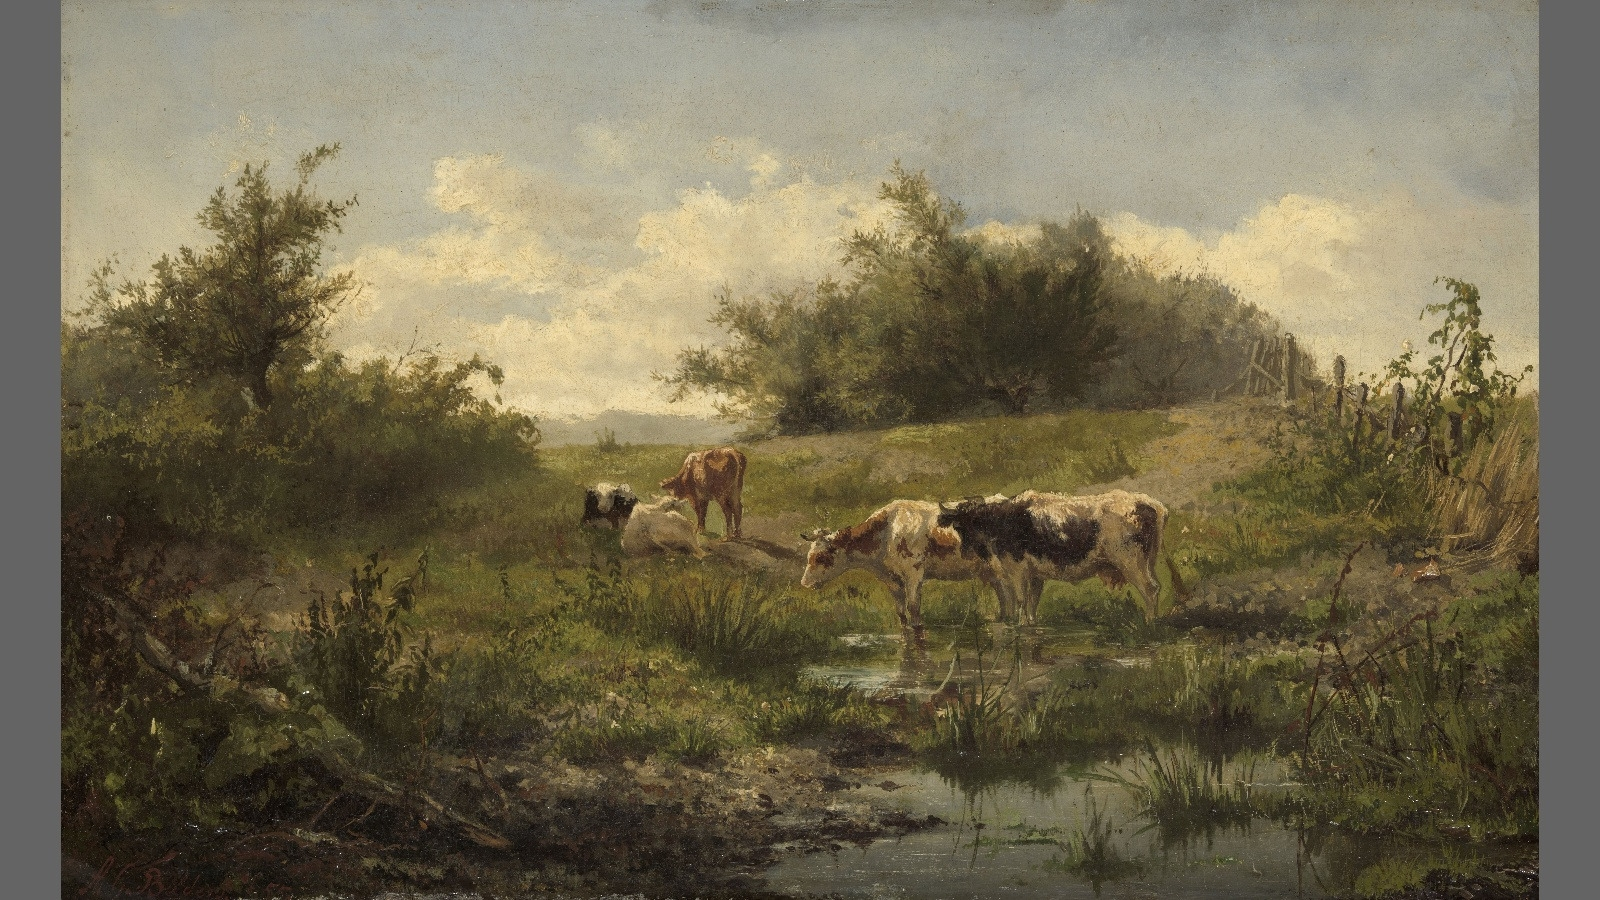
\includegraphics[width=\linewidth]{datas/predictions/stimulus_cows_at_a_pond_Bilders_1856.jpg}
        \caption{}
    \end{subfigure}
    \begin{subfigure}{0.24\textwidth}
        
\includegraphics[width=\linewidth]{datas/predictions/human_cows_at_a_pond_Bilders_1856.jpg}
        \caption{}
    \end{subfigure}

    \begin{subfigure}{0.24\textwidth}
        \includegraphics[width=\linewidth]{datas/predictions/gbvs_cows_at_a_pond_Bilders_1856.jpg}
        \caption{GBVS}
    \end{subfigure}
    \begin{subfigure}{0.24\textwidth}
        \includegraphics[width=\linewidth]{datas/predictions/aws_cows_at_a_pond_Bilders_1856.jpg}
        \caption{AWS}
    \end{subfigure}
    \begin{subfigure}{0.24\textwidth}
        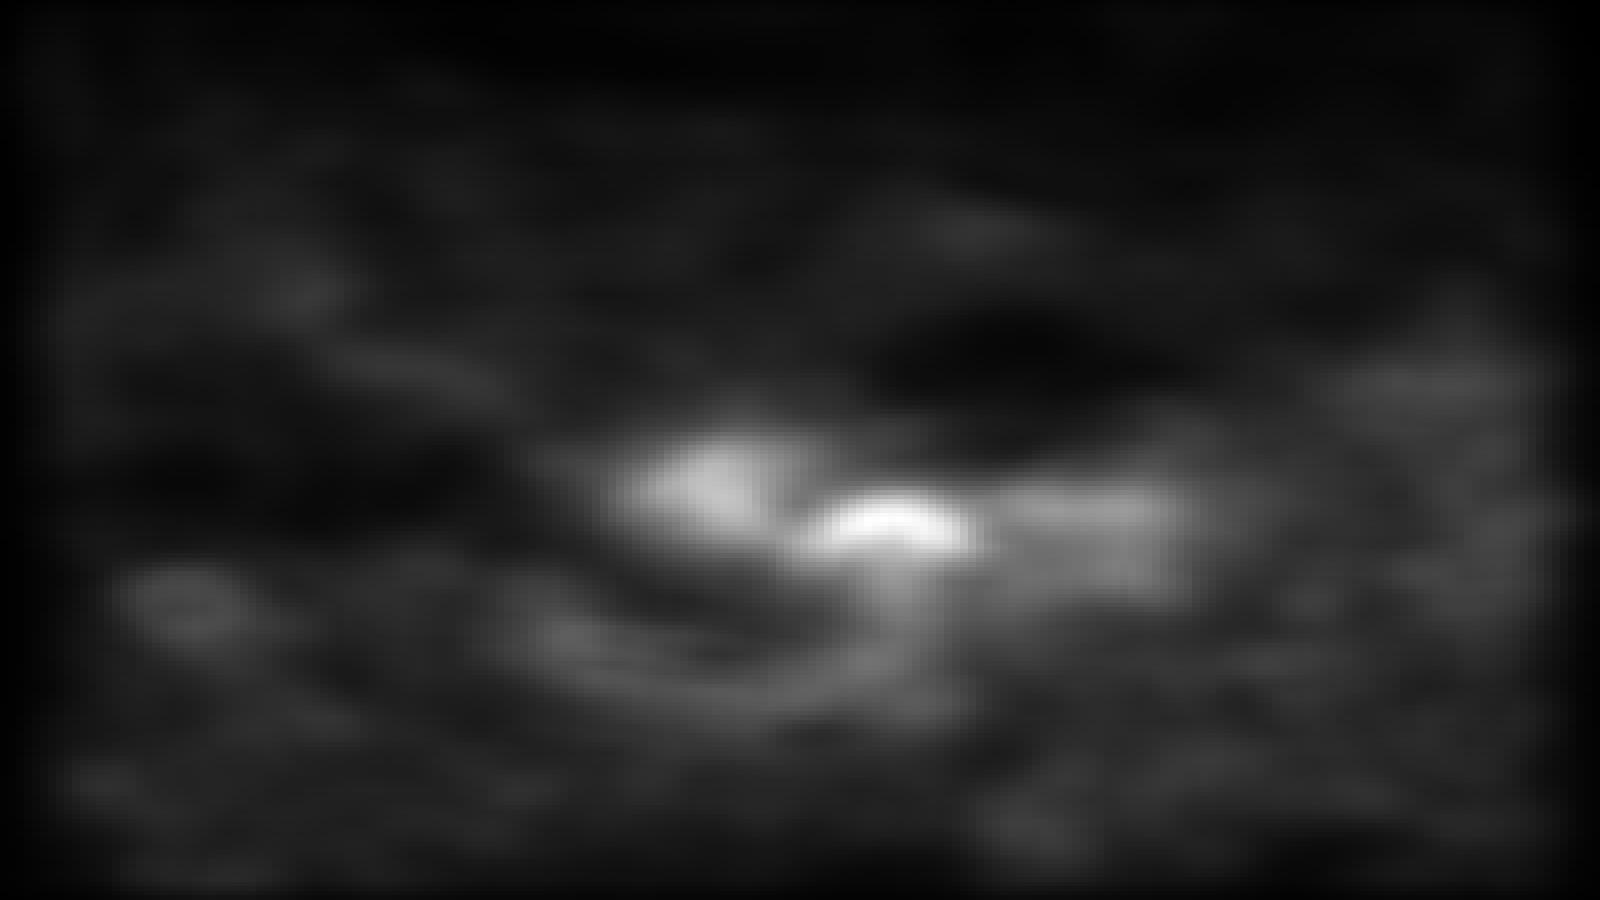
\includegraphics[width=\linewidth]{datas/predictions/rare2012_cows_at_a_pond_Bilders_1856.jpg}
        \caption{RARE2012}
    \end{subfigure}
    \begin{subfigure}{0.24\textwidth}
        \includegraphics[width=\linewidth]{datas/predictions/aim_cows_at_a_pond_Bilders_1856.jpg}
        \caption{AIM}
    \end{subfigure}

    \begin{subfigure}{0.24\textwidth}
        \includegraphics[width=\linewidth]{datas/predictions/mlnet_cows_at_a_pond_Bilders_1856.jpg}
        \caption{MLNET}
    \end{subfigure}
    \begin{subfigure}{0.24\textwidth}
        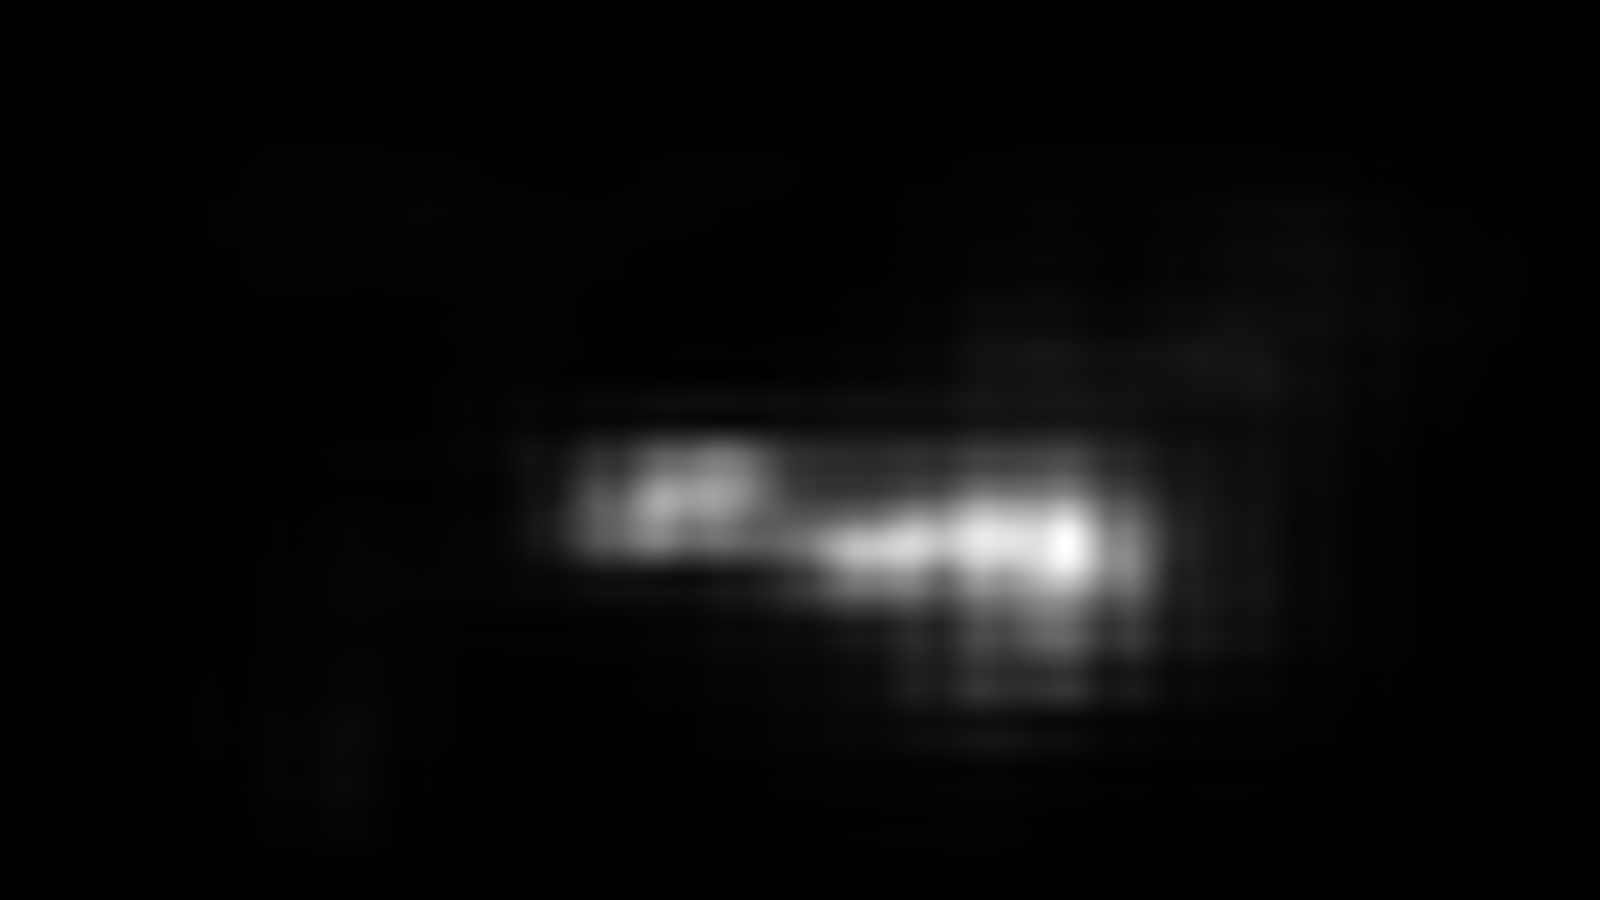
\includegraphics[width=\linewidth]{datas/predictions/SALICON_cows_at_a_pond_Bilders_1856.jpg}
        \caption{SALICON}
    \end{subfigure}
    \begin{subfigure}{0.24\textwidth}
        \includegraphics[width=\linewidth]{datas/predictions/sam_vgg_cows_at_a_pond_Bilders_1856.jpg}
        \caption{SAM-VGG}
    \end{subfigure}
    \begin{subfigure}{0.24\textwidth}
        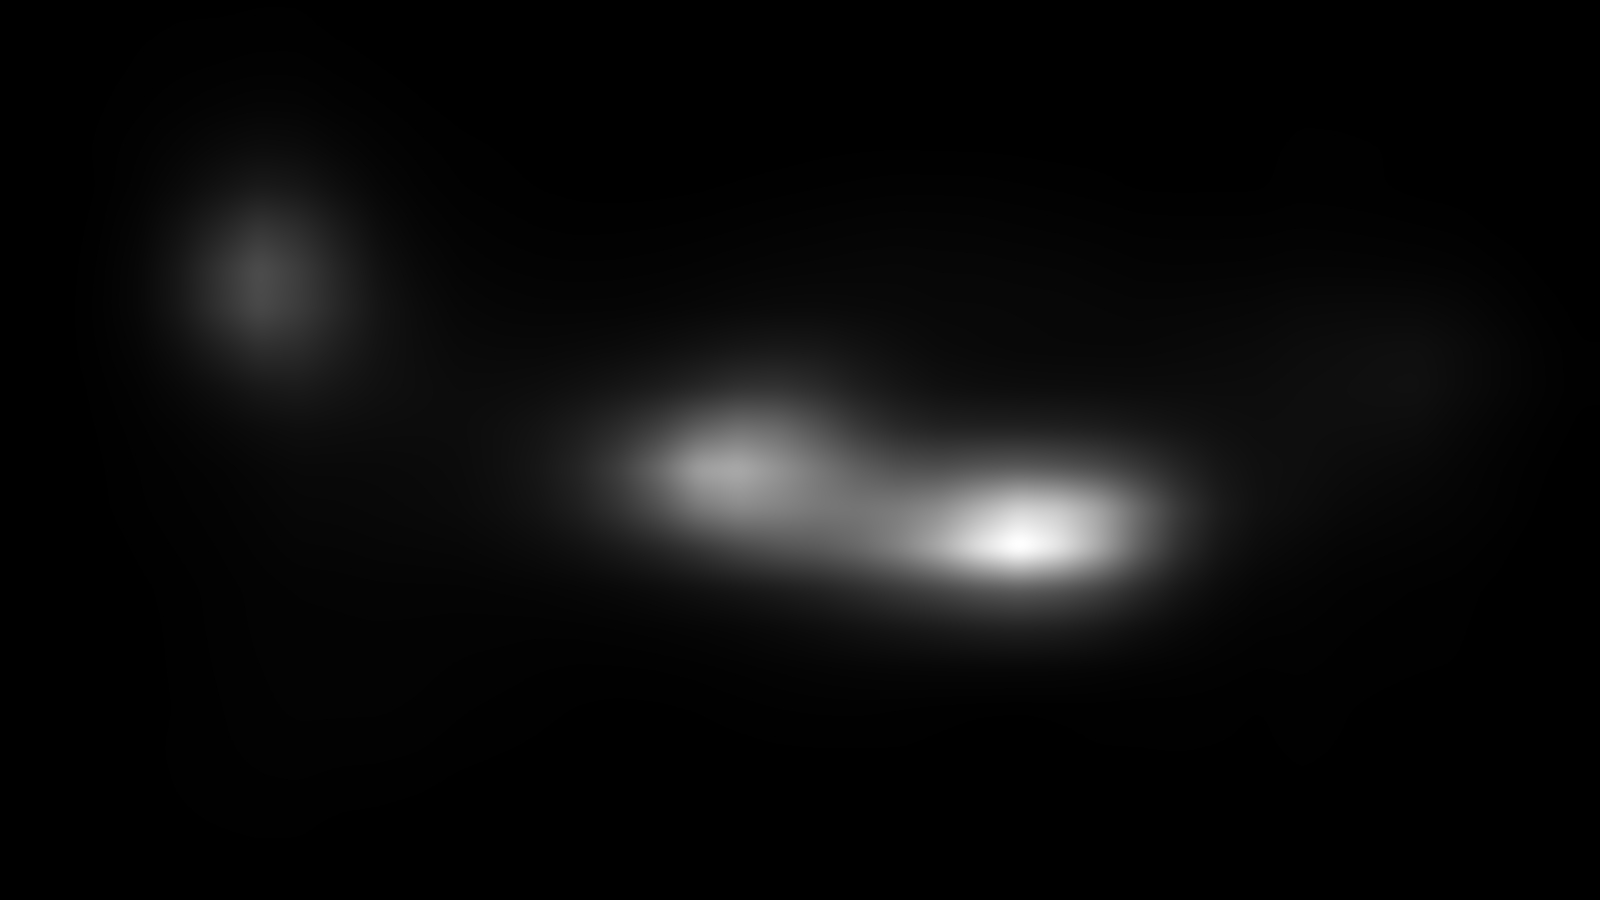
\includegraphics[width=\linewidth]{datas/predictions/sam_resnet_cows_at_a_pond_Bilders_1856.jpg}
        \caption{SAM-ResNet}
    \end{subfigure}
     
    \caption{Cartes de saillance de modèles fait-mains (2\up{ème} ligne) et profonds (3\up{ème} ligne). La 1\up{ère} ligne illustre le stimuli originale et sa carte de saillance humaine}
    \label{fig:saliencyModel}
\end{figure}

\vfill

\begin{table}[ht]
    \centering
        \begin{tabular}{|l|l|l|l|l|l|l|}
		\hline
        Modèle & CC~$\uparrow$ & KL~$\downarrow$ & SIM~$\uparrow$ & NSS~$\uparrow$ & AUC-B~$\uparrow$ & AUC-J~$\uparrow$\\
		\hline
        GBVS        & 0.506 & 0.962 & 0.446 & 1.256 & \textbf{0.809} & 0.817\\
        RARE2012    & 0.443 & 1.020 & 0.438 & 1.103 & 0.777 & 0.786\\
        AIM         & 0.315 & 1.245 & 0.371 & 0.772 & 0.723 & 0.735\\
        AWS         & 0.427 & 1.045 & 0.430 & 1.083 & 0.762 & 0.769\\
		\hline
        Moyenne     & 0.422 & 1.068 & 0.421 & 1.053 & 0.774 & 0.776\\
		\hline
        MLNET       & 0.576 & \textbf{0.832} & 0.513 & 1.524 & 0.770 & 0.818\\
        DeepGazeII  & 0.485 & 0.896 & 0.488 & 1.394 & 0.679 & 0.804\\
        SALICON     & 0.538 & 0.880 & 0.517 & 1.445 & 0.708 & 0.827\\
        SAM ResNet  & \textbf{0.700} & 0.984 & \textbf{0.613} & \textbf{1.834} & 0.782 & \textbf{0.862}\\
        SAM VGG     & 0.617 & 0.970 & 0.561 & 1.603 & 0.752 & 0.846\\
		\hline
        Moyenne     & 0.583 & 0.912 & 0.551 & 1.560 & 0.738 & 0.831\\
		\hline
        \end{tabular}
    \caption{Performances des modèles de saillance sur les peintures de la base de données.}
    \label{tab:scores}
\end{table}

\vfill

% \newpage
\section{Entrainement du modèle}
